\documentclass{article}
\usepackage{cite}
\usepackage{color}
\usepackage{fullpage}
\usepackage{pgf}
%\usepackage{hyperref}
\usepackage[normalem]{ulem}
\newcommand{\jri}[1]{\textcolor{blue}{\emph{#1}} }
\newcommand{\citex}{\textcolor{blue}{\bf CITE}}
\newcommand{\X}{\textcolor{blue}{\bf X}}

\begin{document}

\title{Supporting Information: Demographic history and patterns of selection in maize during and since domestication}
\author{Timothy M. Beissinger, Li Wang, Arun Durvasula, Kate Crosby, \\ Matthew Hufford, Jeffrey Ross-Ibarra}

\maketitle
\section*{}


\begin{figure}[h!]
  \begin{center}
    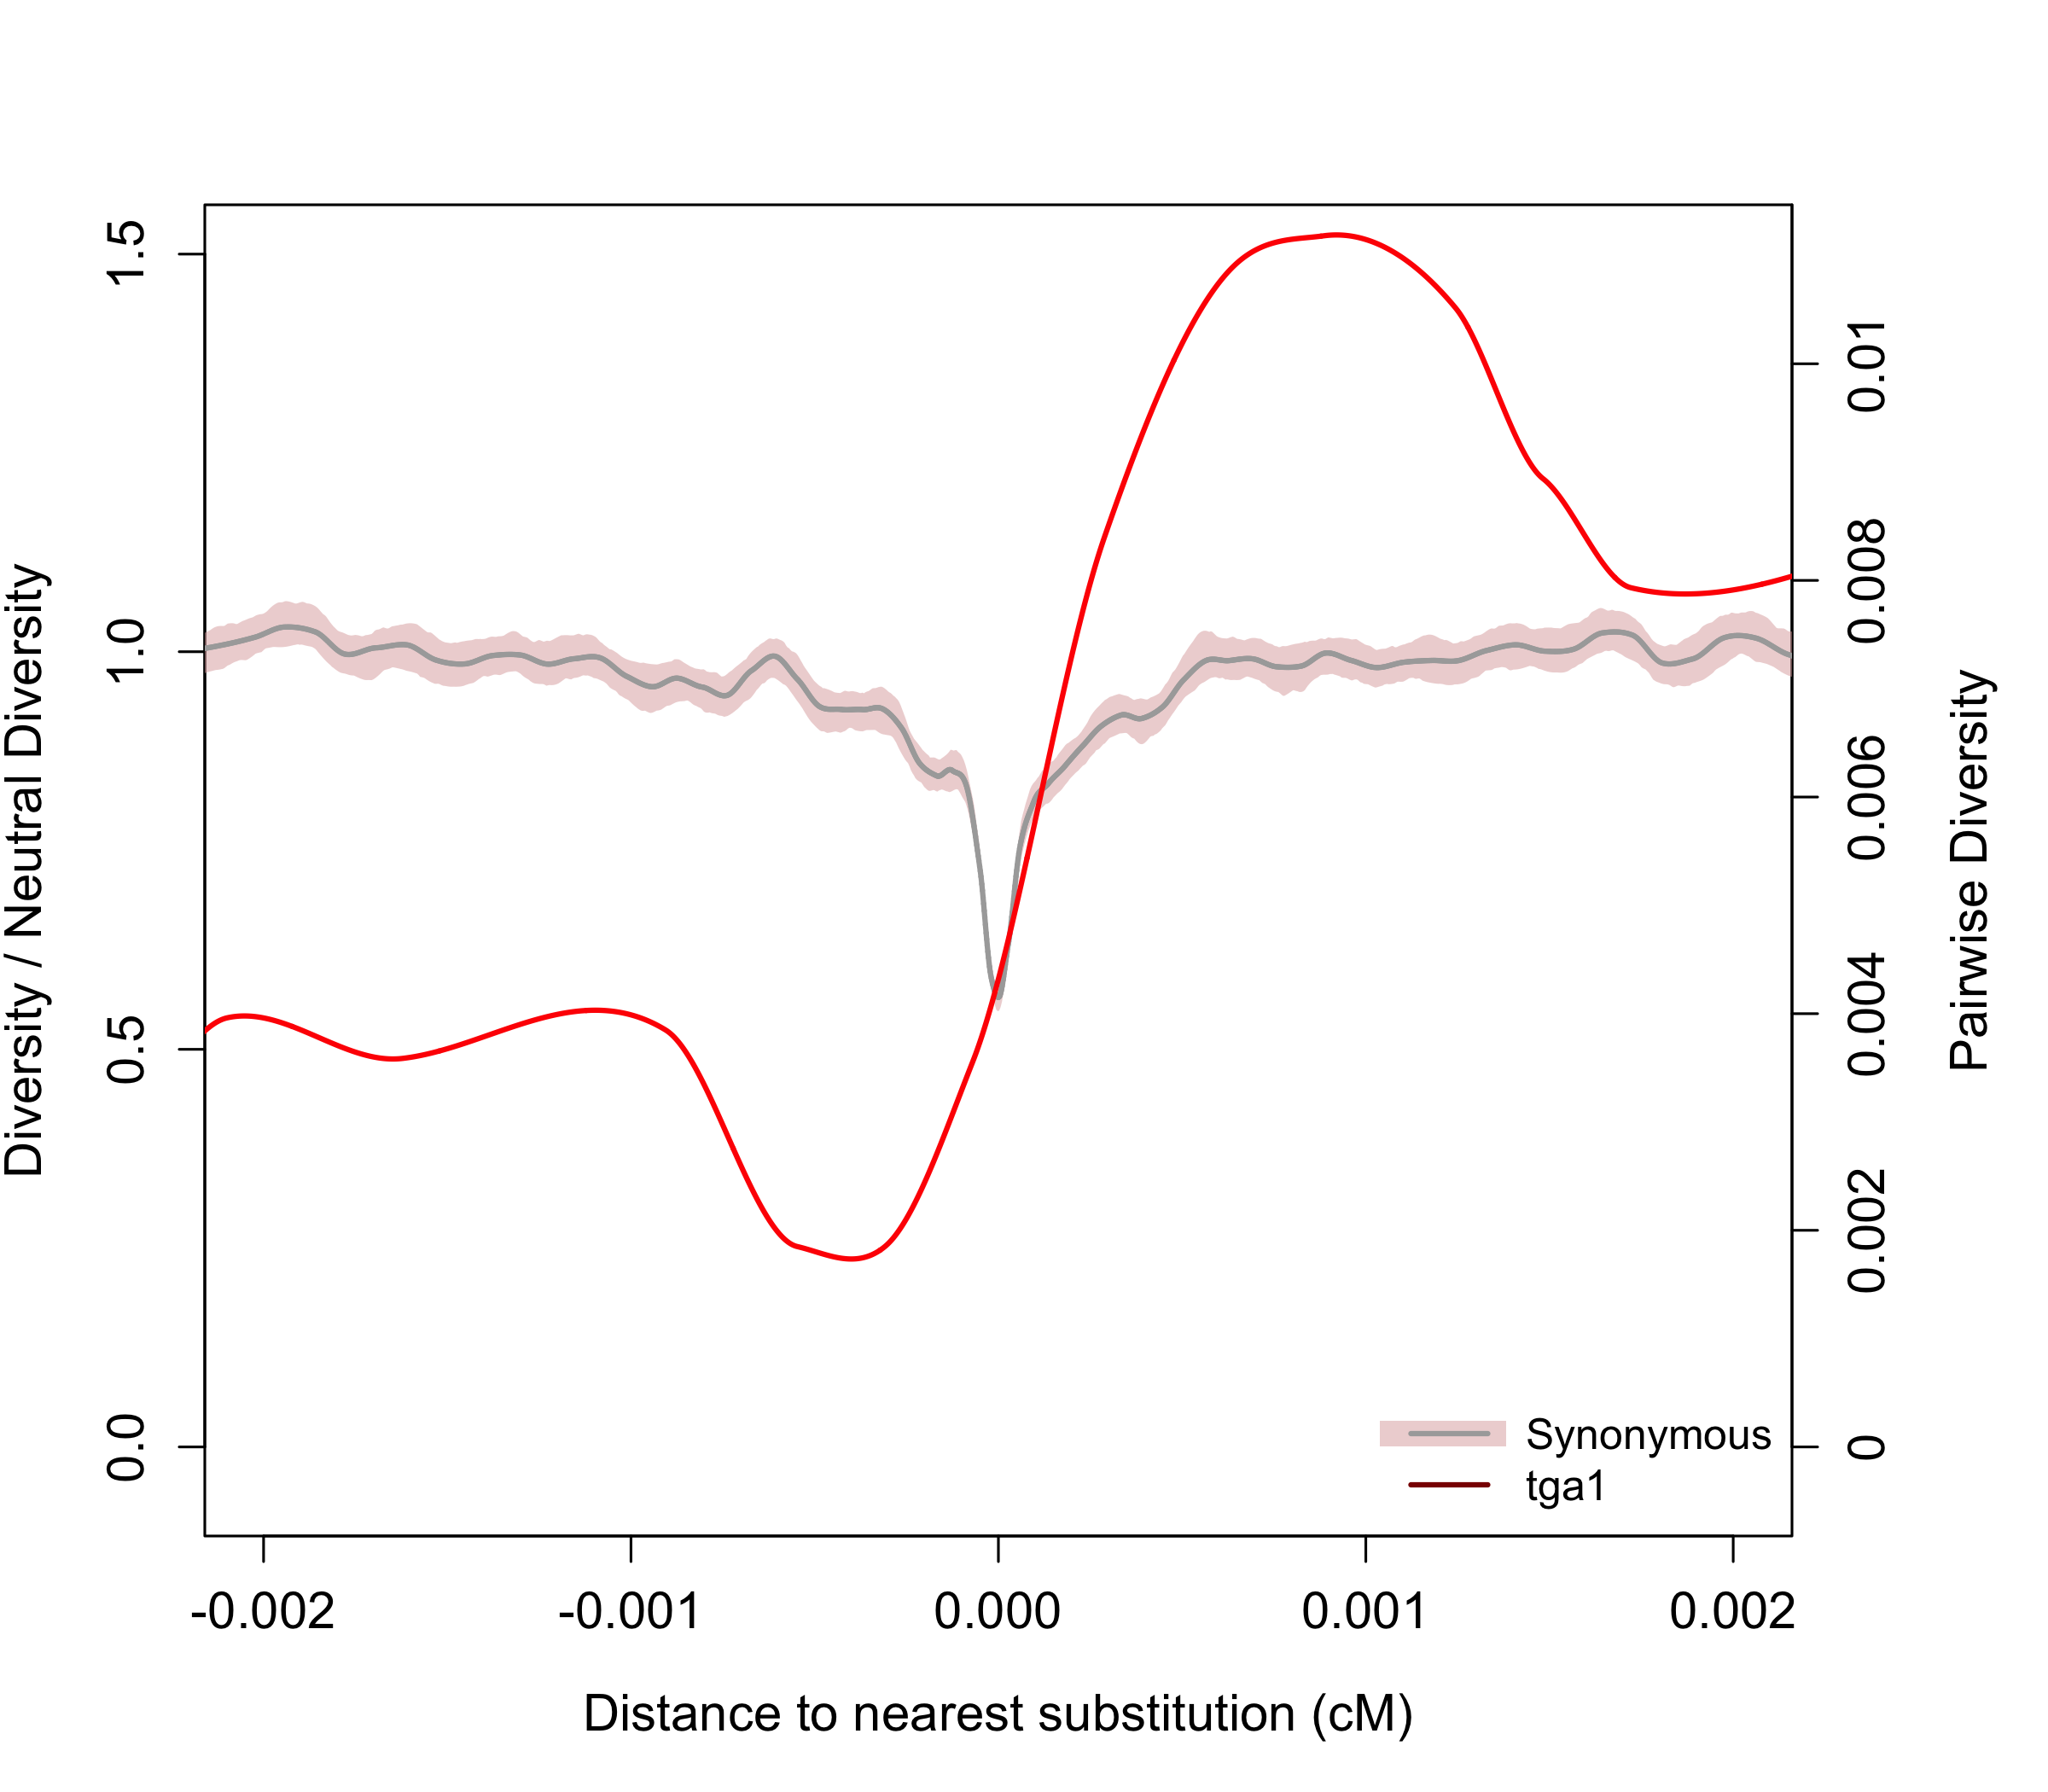
\includegraphics[width=.85\textwidth]{FigsAndFiles/plotDiversity_TvM_Folded2_Significance_tga1Supp_June.png} \\
    \end{center}
{\bf Figure S1:} Diversity surrounding the causitive polymorphism at the \emph{tga1} locus is plotted. Since this is only one gene, the large amount of noise compared to our average plots is expected. However, notice that diversity precisely at the causitive polymorphism is reduced and a recovery of diversity is observed away from that site.
\end{figure}


\begin{figure}[h!]
  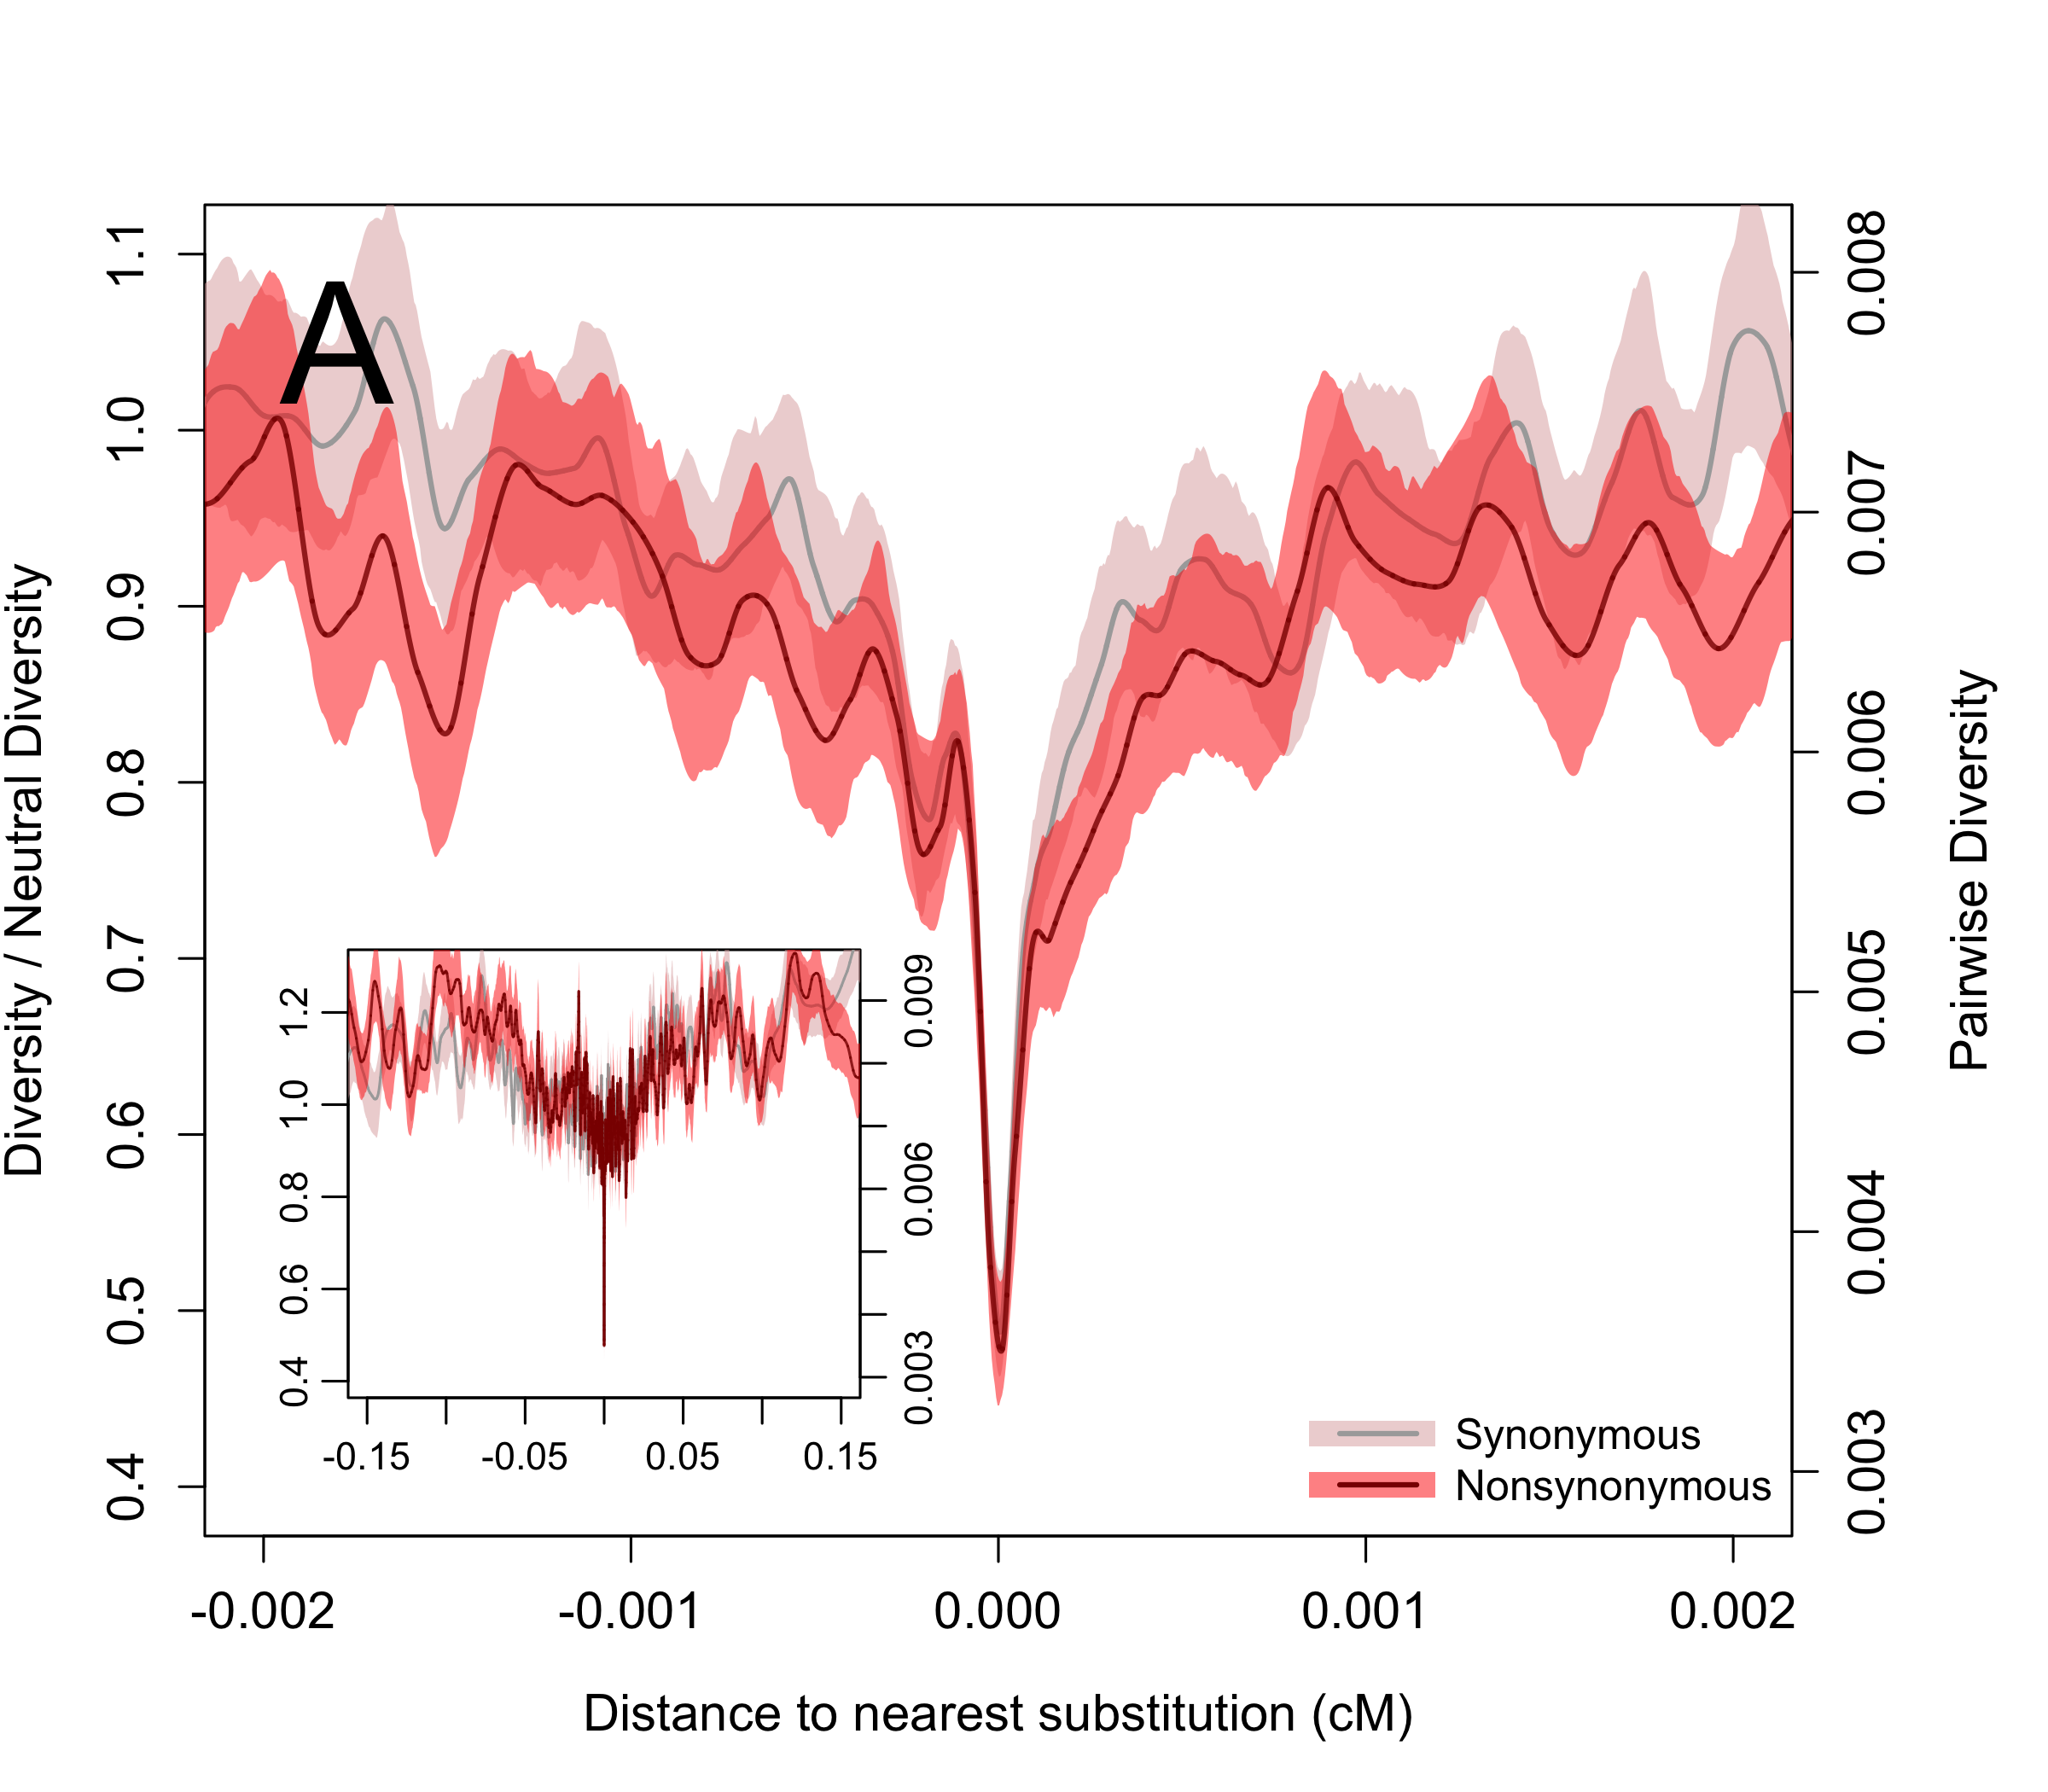
\includegraphics[width=.5\textwidth]{FigsAndFiles/plotDiversity_TvM_Conserved_Significance_June.png}
  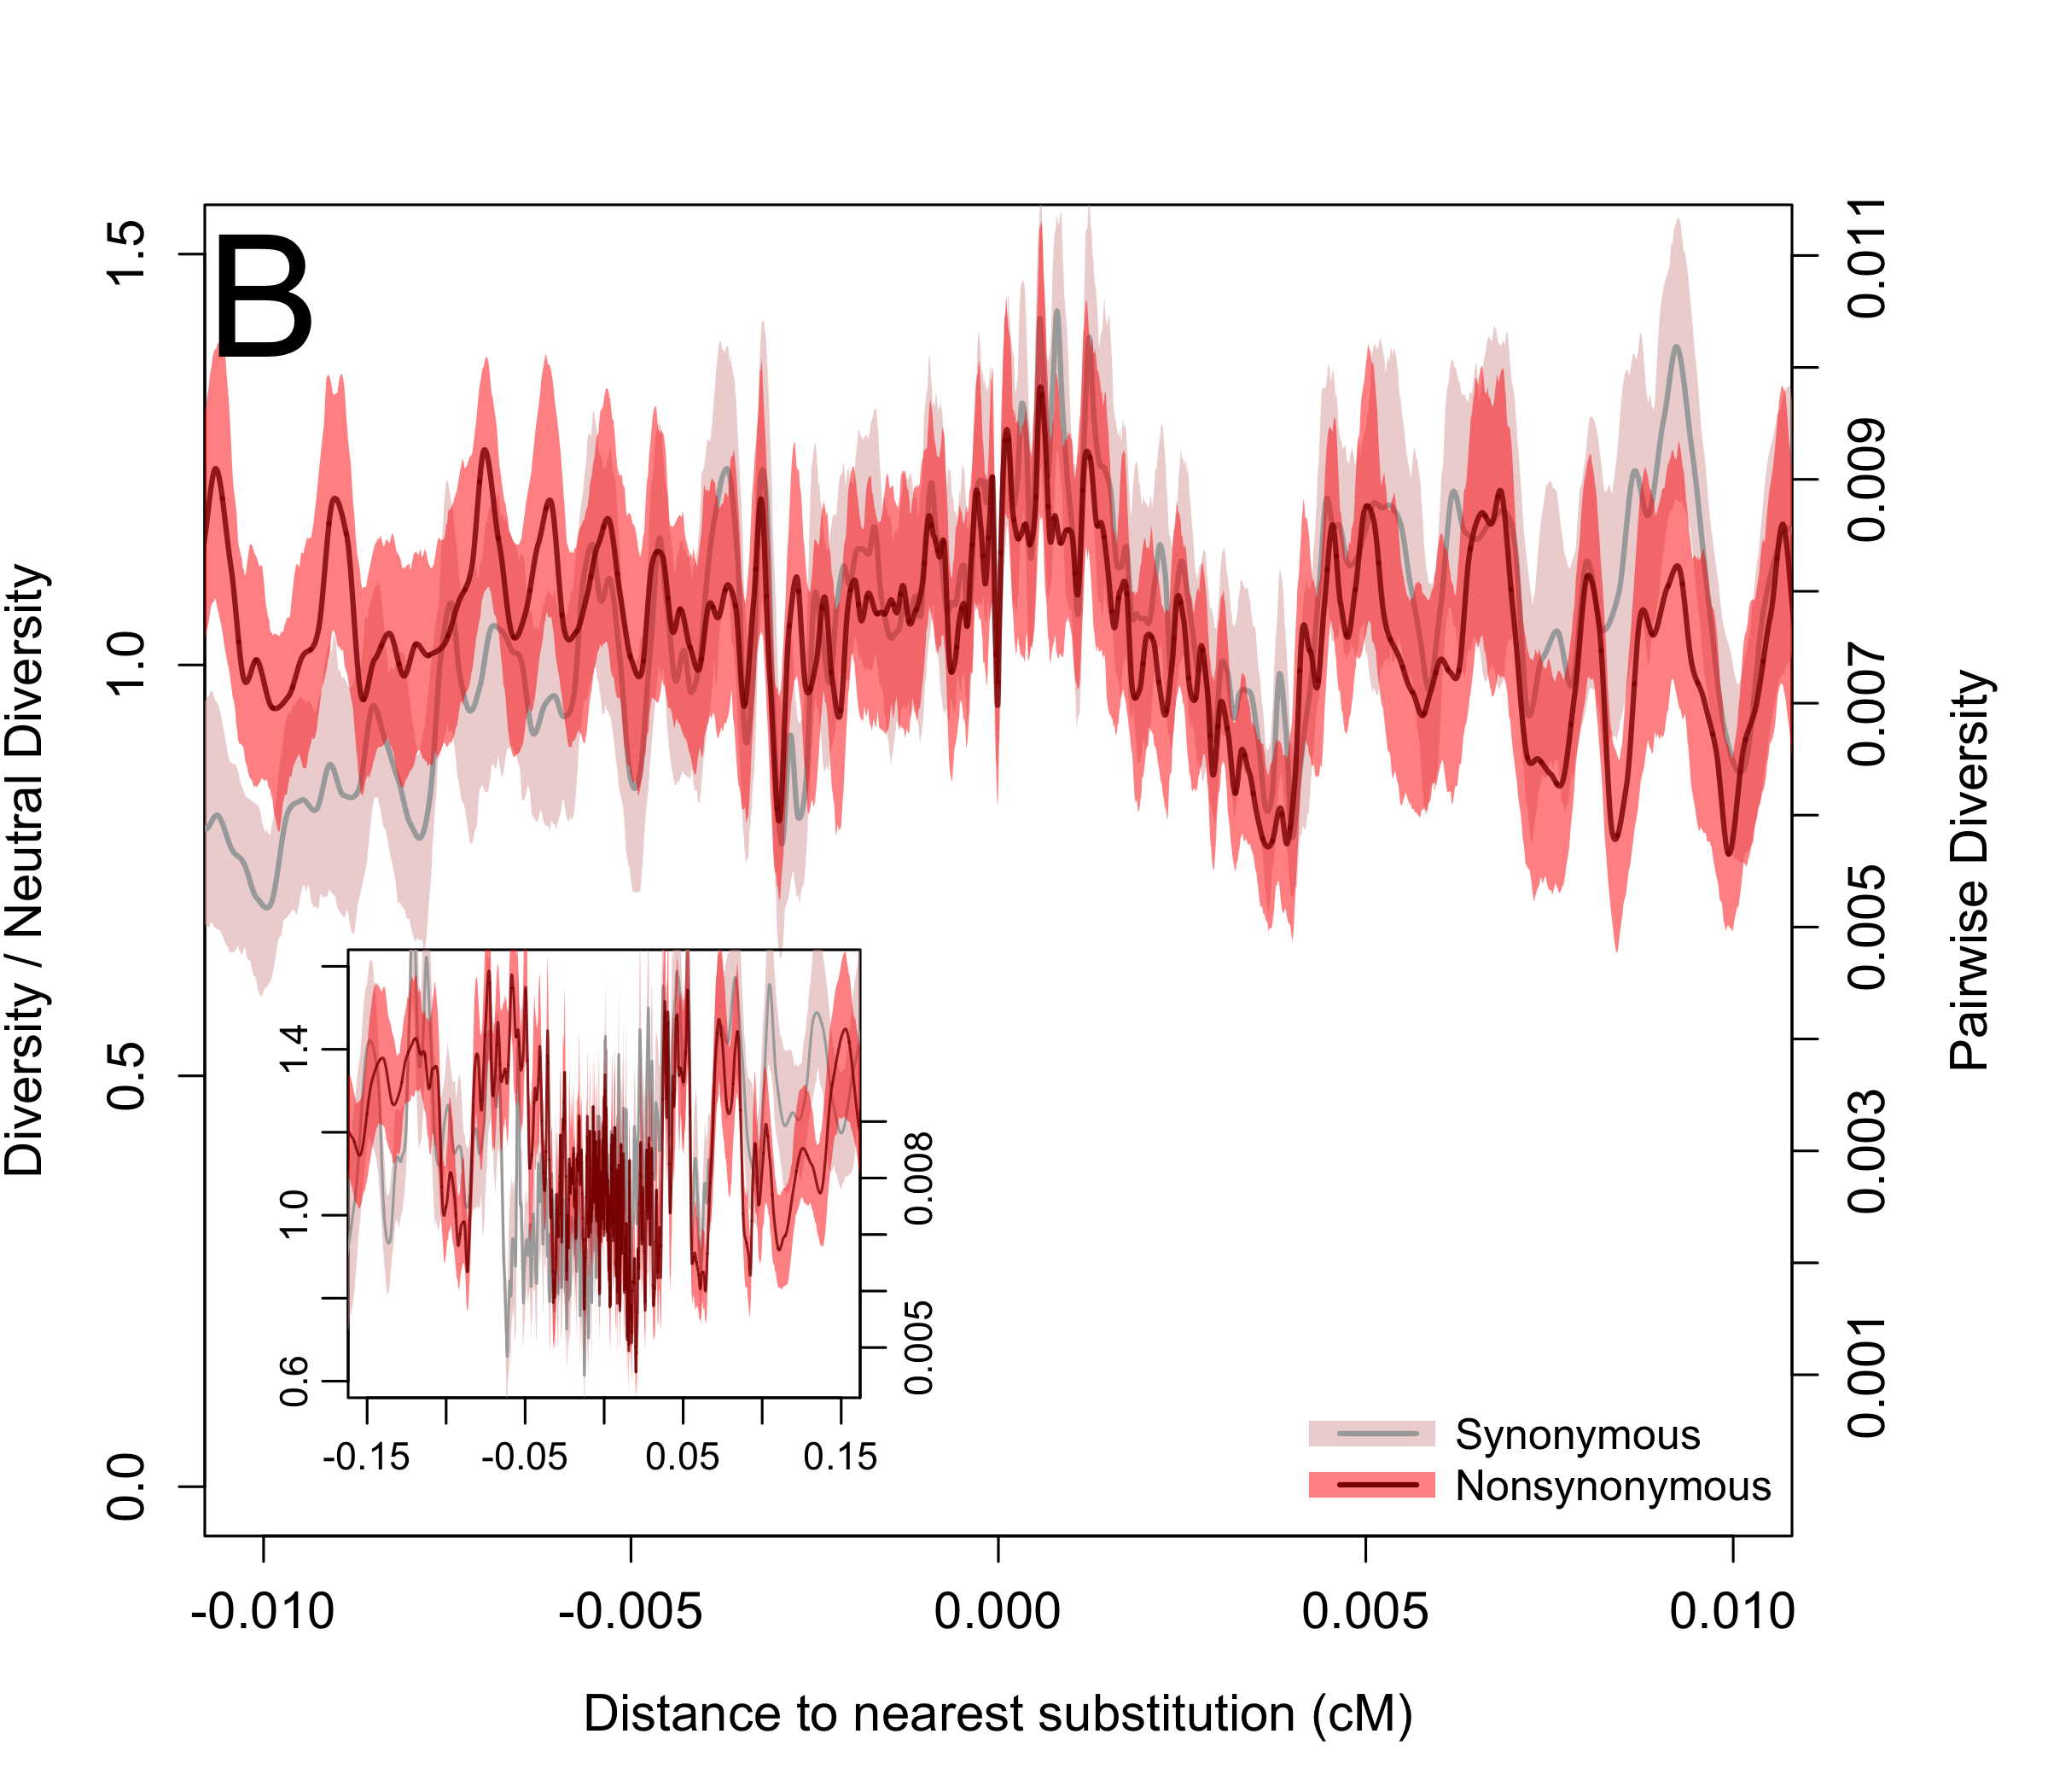
\includegraphics[width=.5\textwidth]{FigsAndFiles/plotDiversity_TvM_Unconserved_Significance_June.png}
{\bf Figure S2:} Pairwise diversity surrounding synonymous and nonsynonymous
  substitutions in maize at highly conserved (A) or unconserved (B) sites.  Bootstrap-based 95\% confidence intervals are depicted via shading. Inset plots depict a larger range on the x-axis.
\end{figure}


\begin{figure}[h!]
  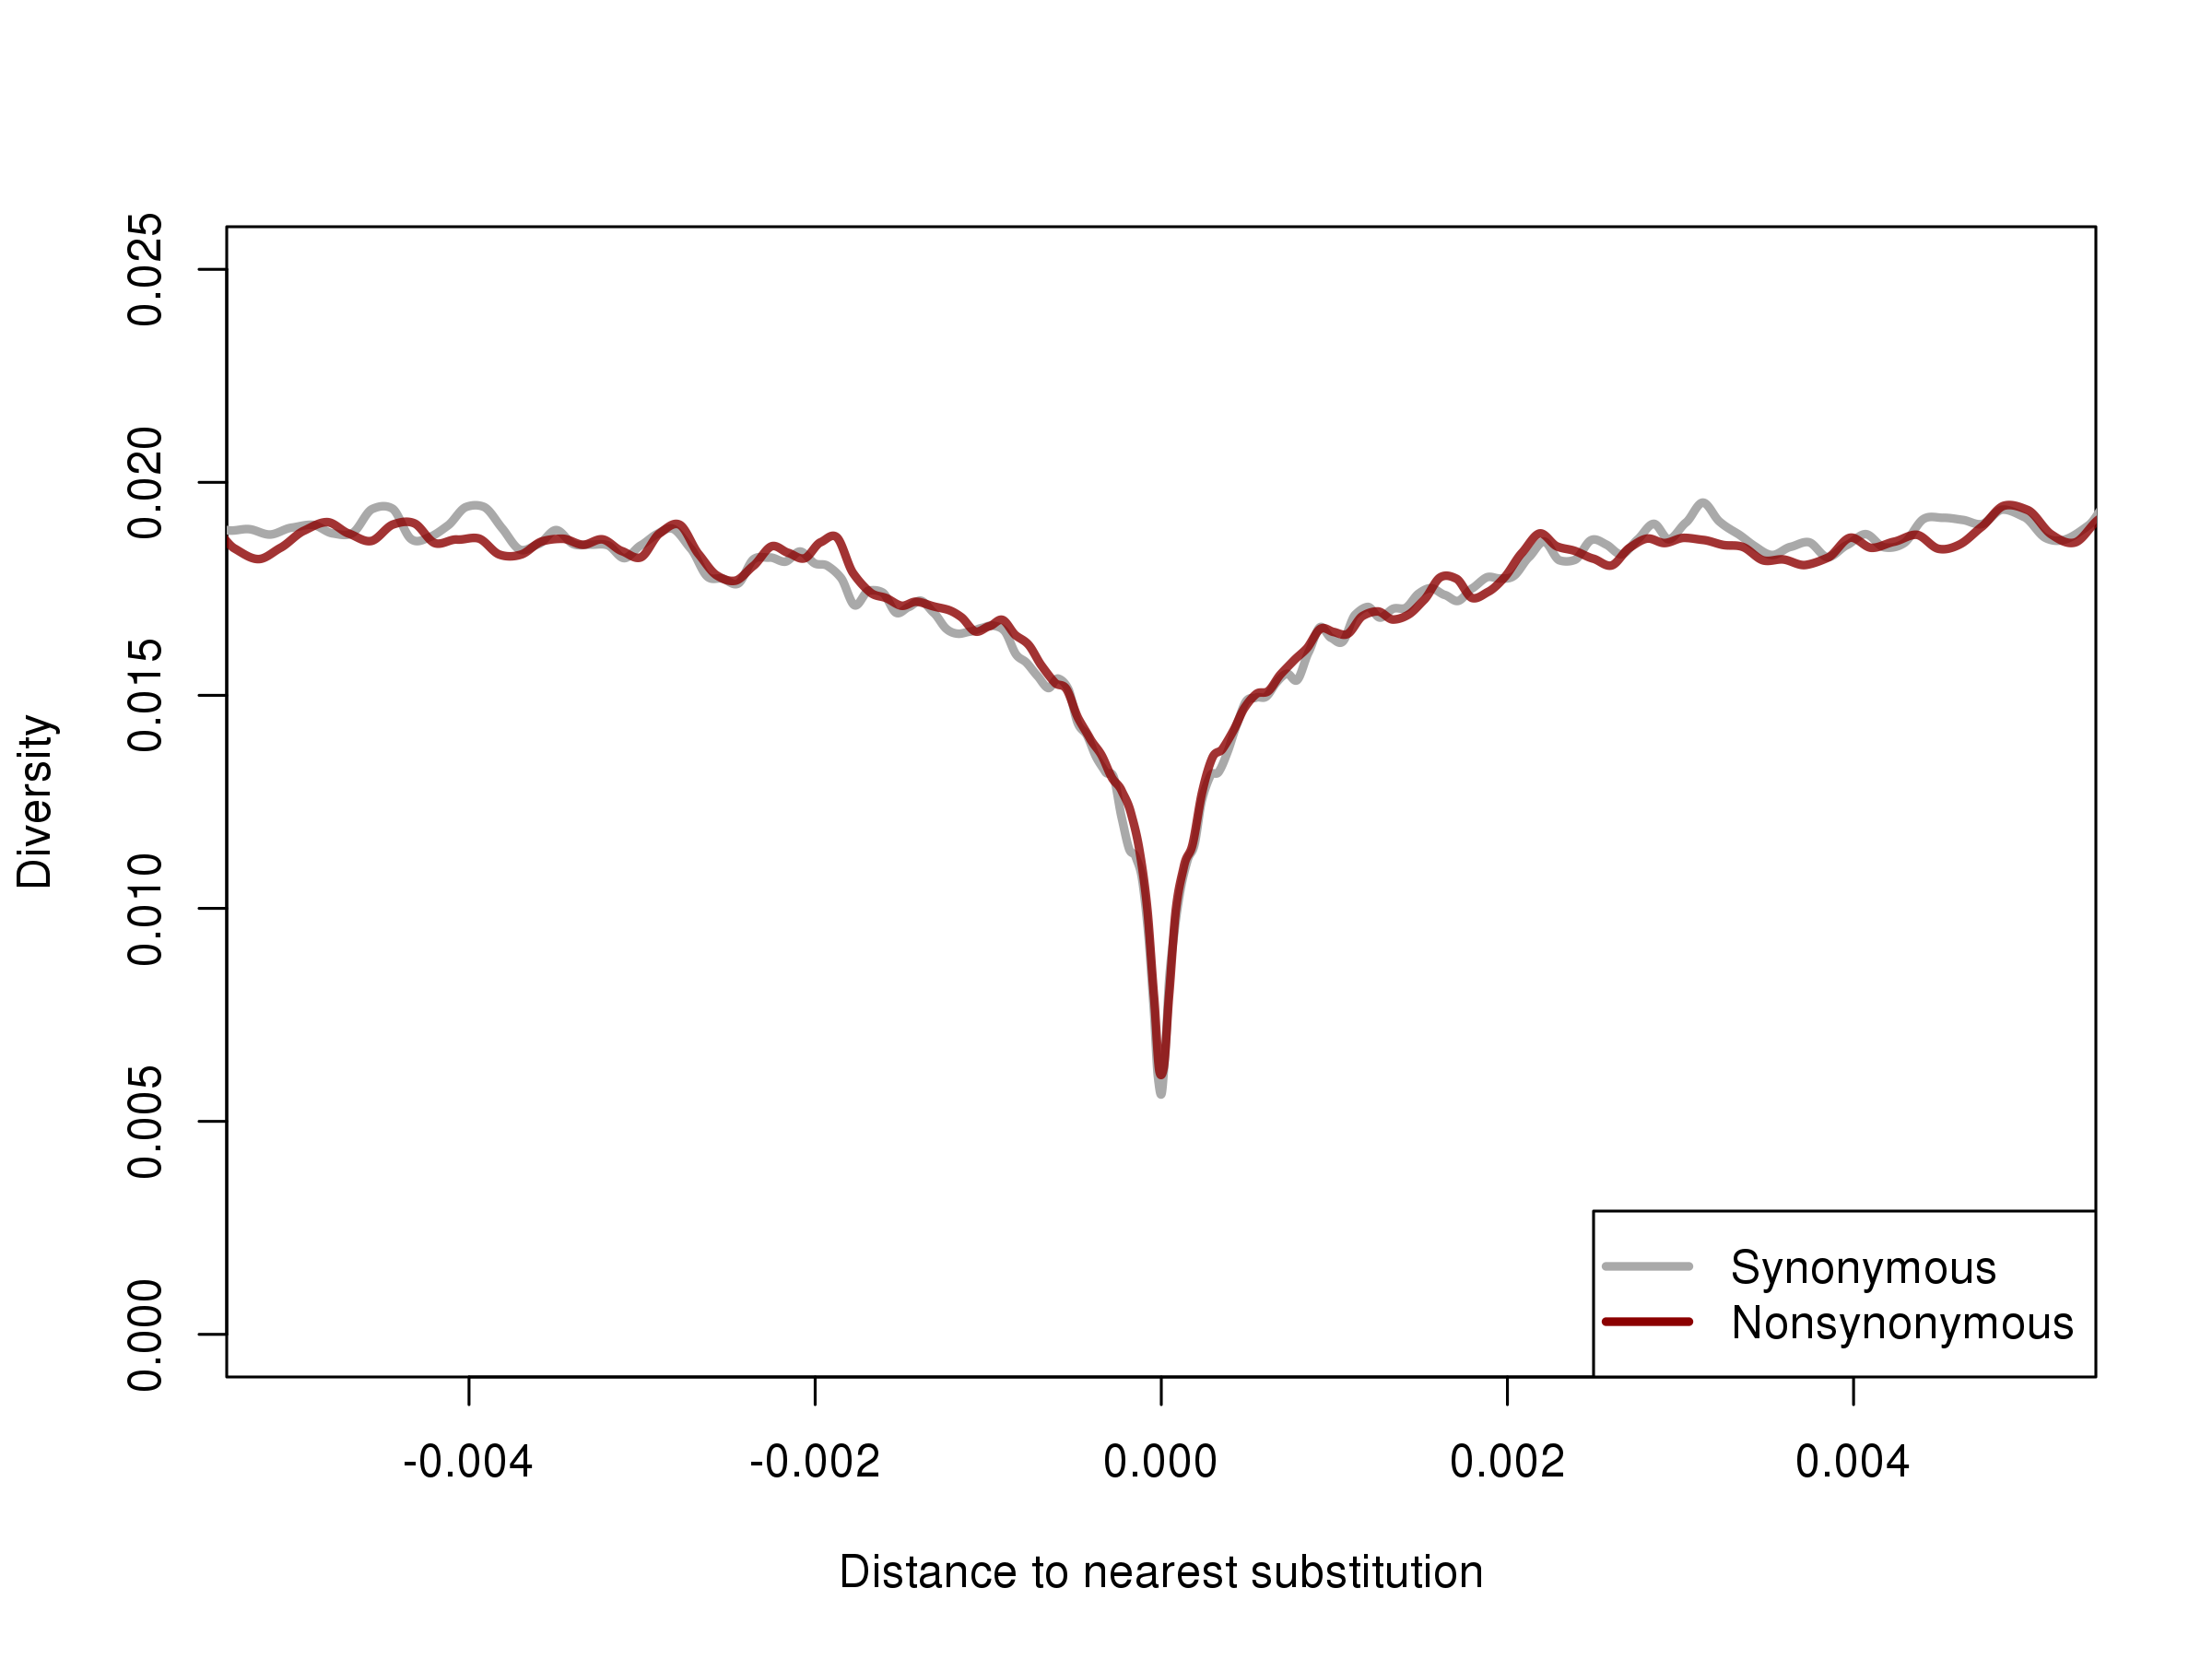
\includegraphics[width=\textwidth]{FigsAndFiles/plotDiversity_TvM_Singletons.png}
{\bf Figure S3:} Singleton diversity surrounding synonymous and nonsynonymous
  substitutions in maize.
\end{figure}


\begin{figure}[h!]
  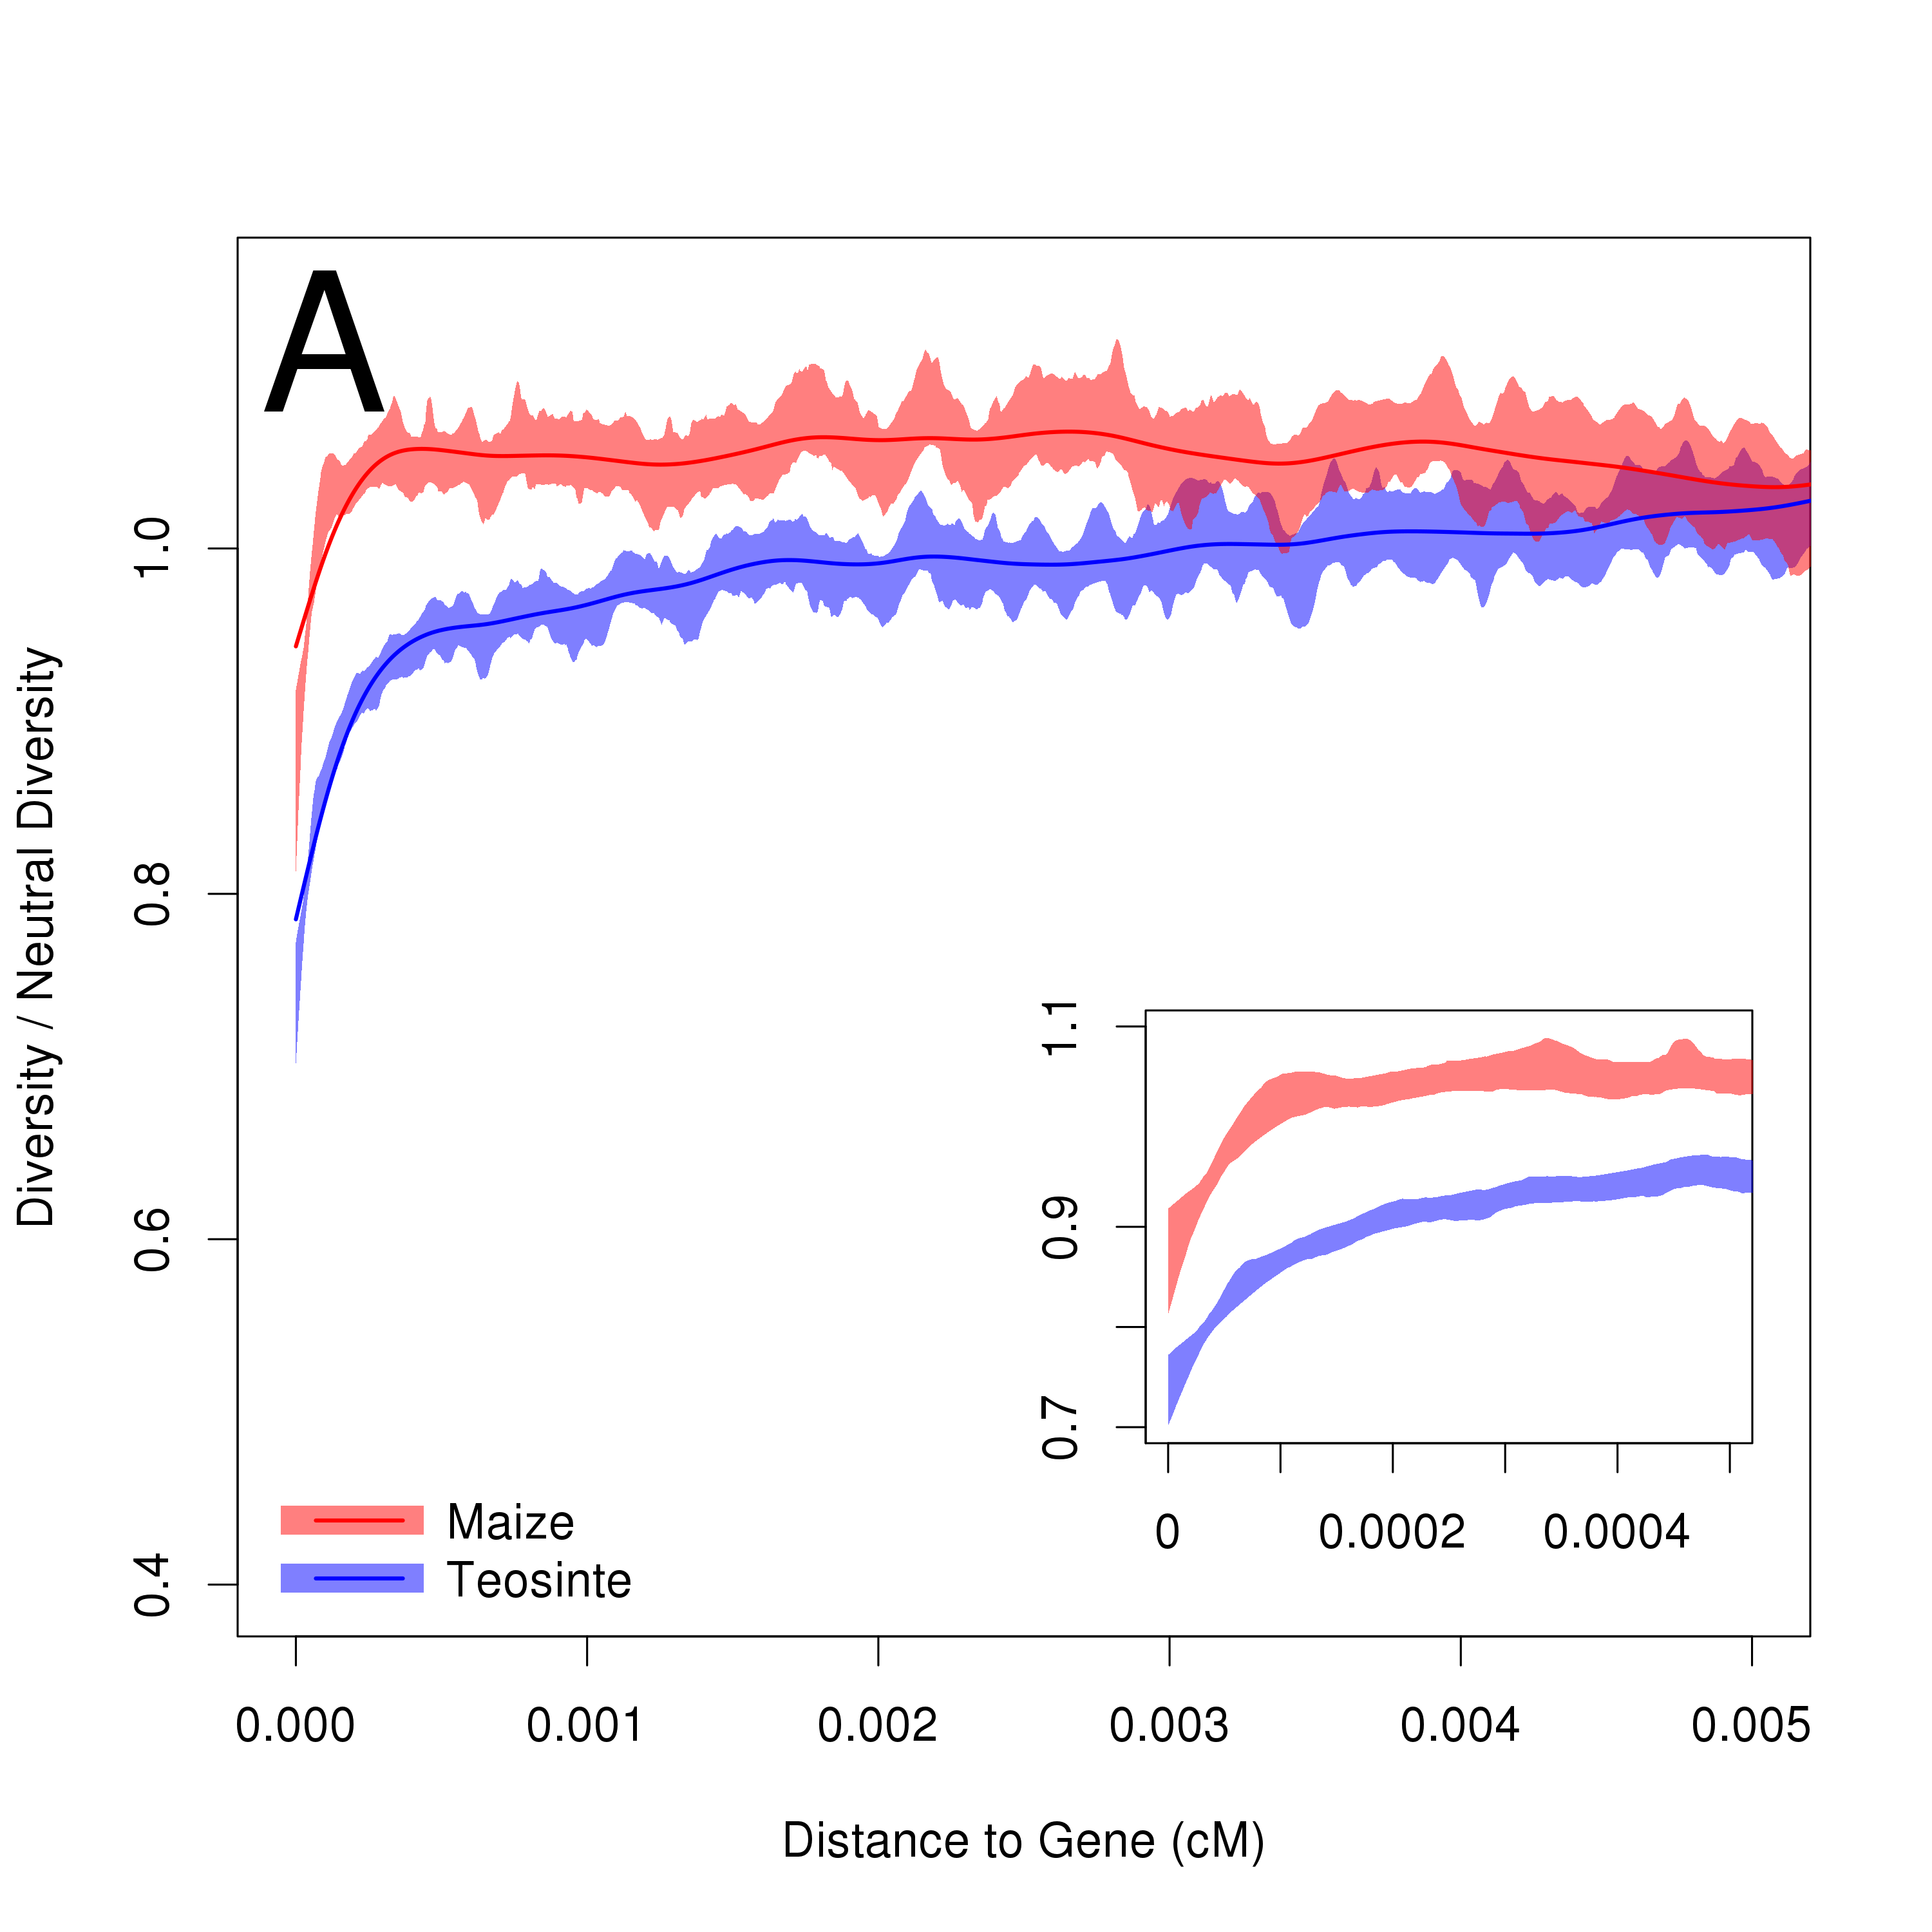
\includegraphics[width=.5\textwidth]{FigsAndFiles/distanceToGene_Unselected_manuscript.png}
    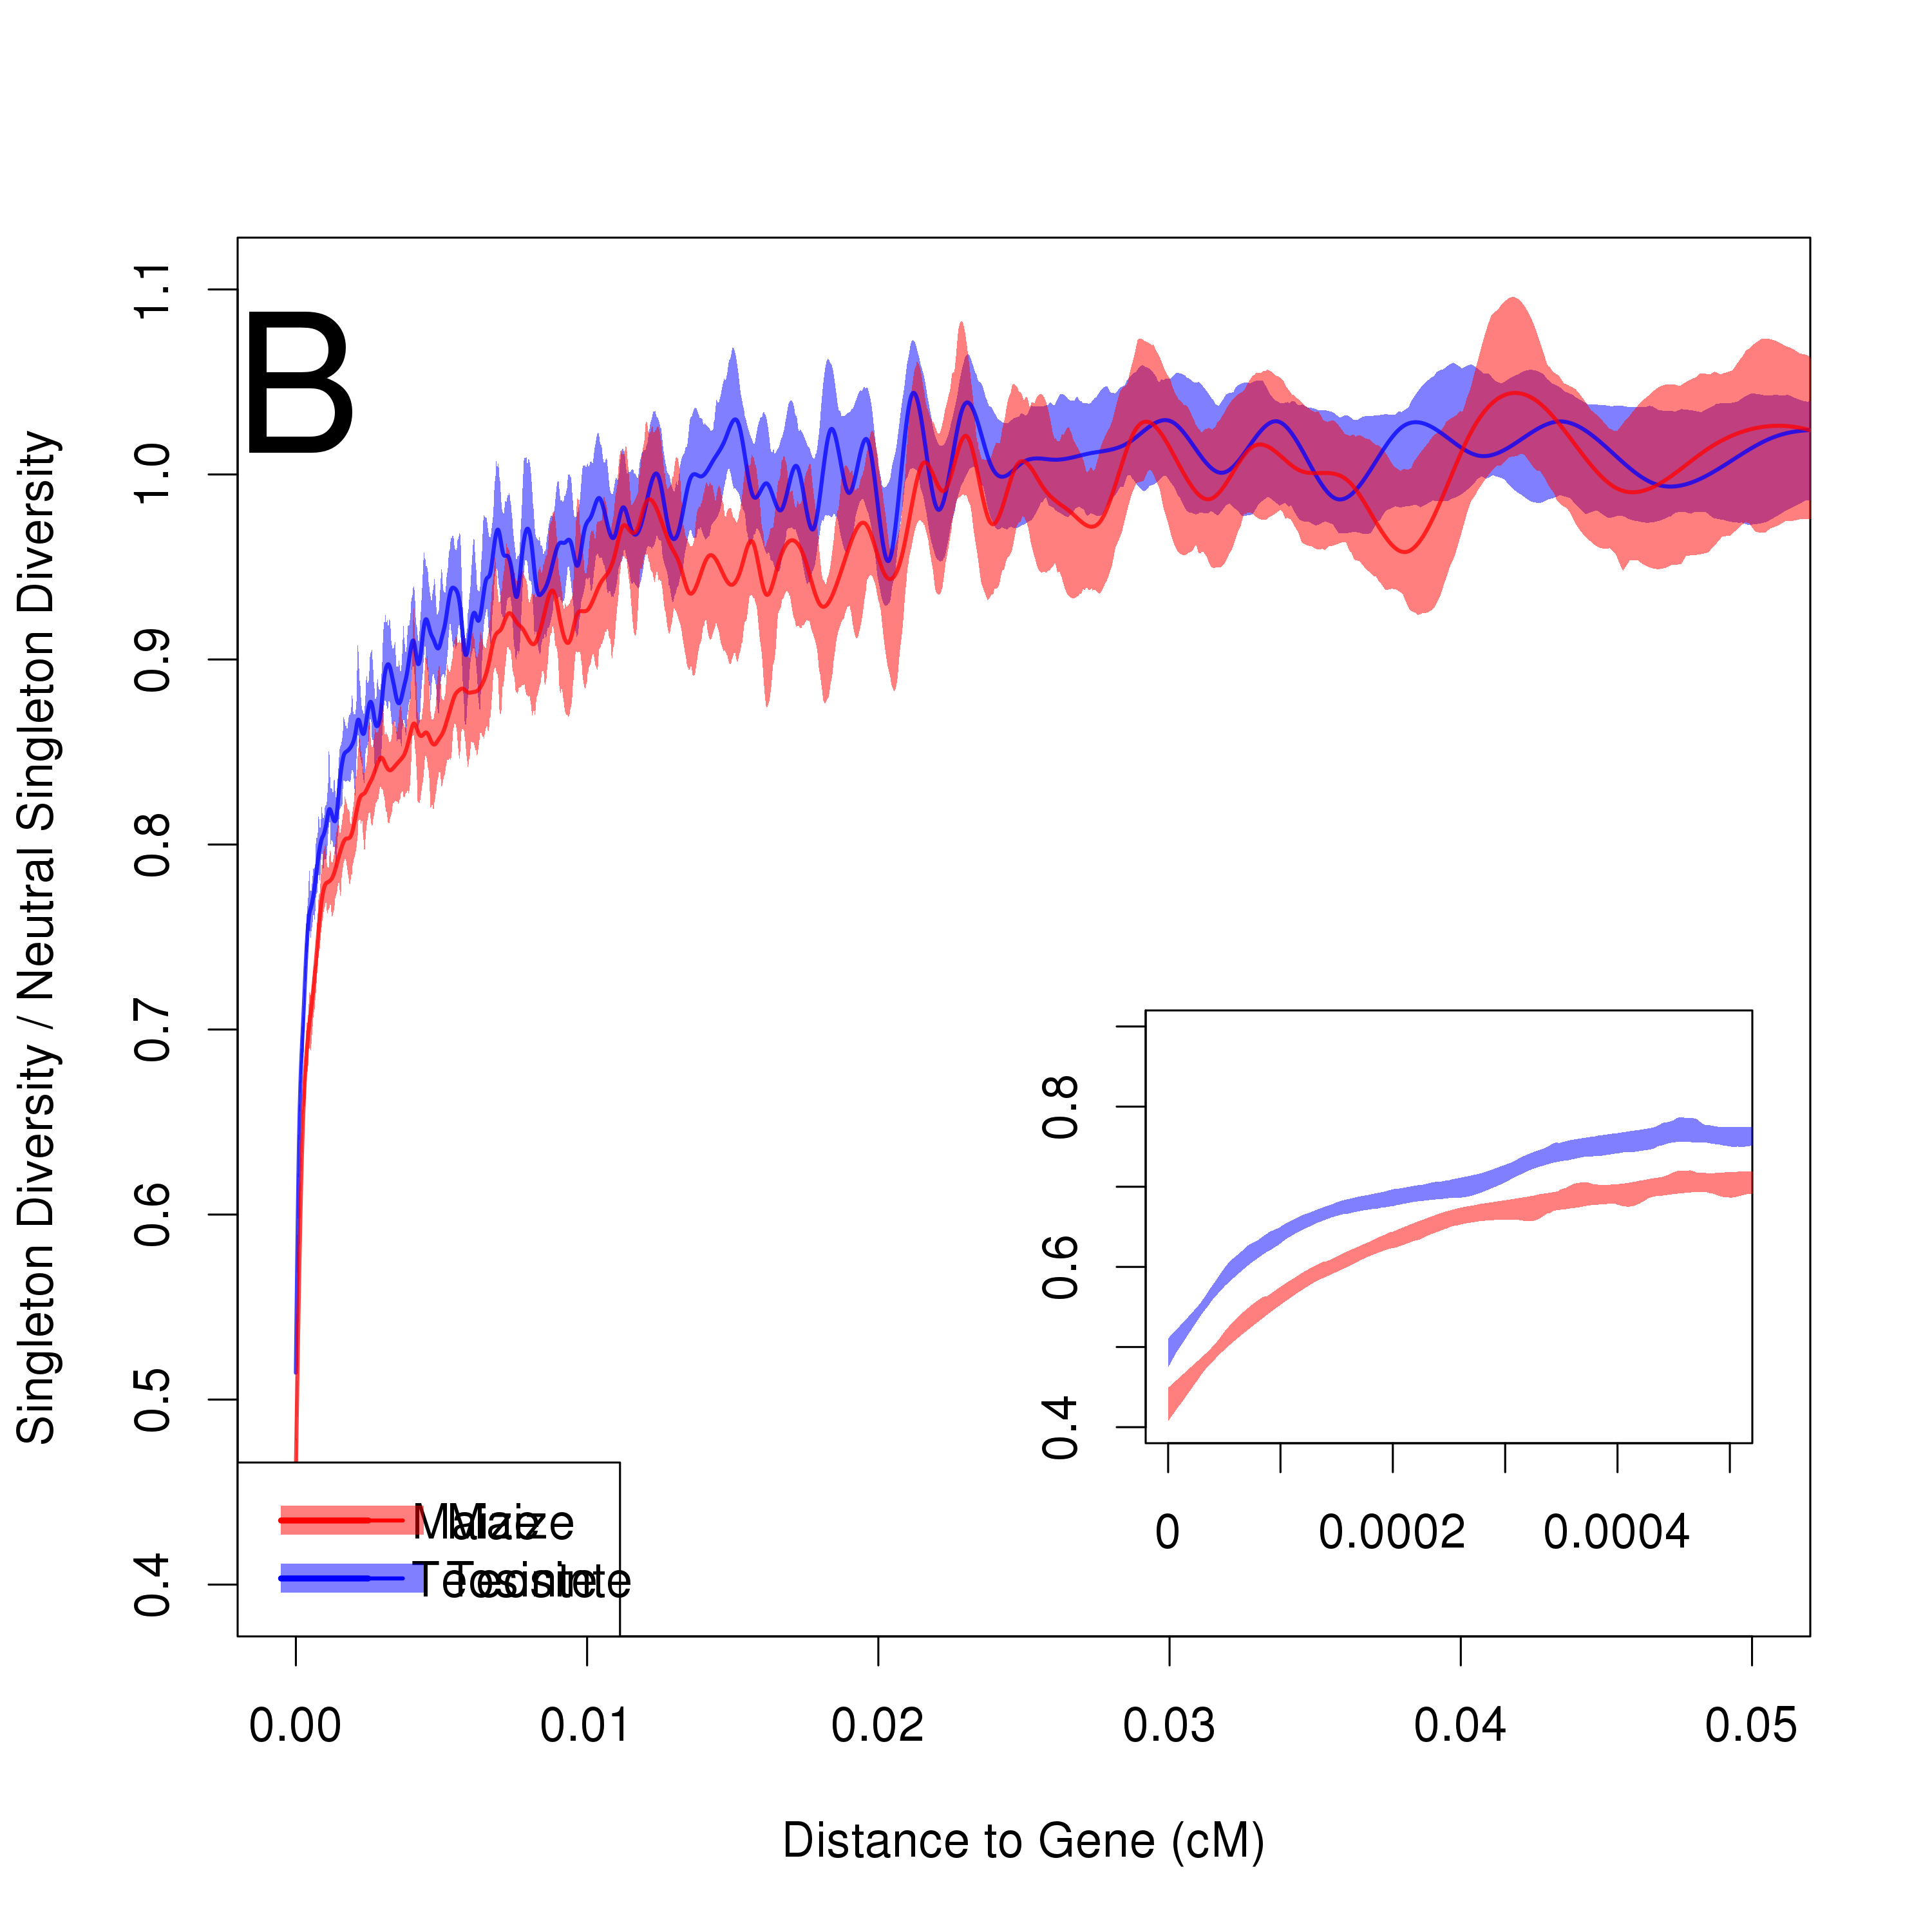
\includegraphics[width=.5\textwidth]{FigsAndFiles/distanceToGene_unselected_Singletons_manuscript.png}
{\bf Figure S4:} Relative level of diversity versus distance to the nearest gene, in maize and teosinte, based on only sites that do not show evidence of hard or soft sweeps according to H12. Two measures of diversity were investigated. {\bf A} displays pairwise diversity,
which is most influenced by intermediate frequency alleles and therefore depicts more ancient evolutionary patterns, and {\bf B} depicts singleton diversity, influenced by rare alleles
and thus depicting evolutionary patterns in the recent past. Bootstrap-based 95\% confidence intervals are depicted via shading. Inset plots depict a smaller range on the x-axis.
\end{figure}


\end{document}
